\documentclass[aspectratio=169,10pt]{beamer}

% ------------------------------------------------------------------------------
% CONFIGURATION DU THÈME & COULEURS AMA
% ------------------------------------------------------------------------------
\usetheme{Madrid}
\usecolortheme{default}

\usepackage[utf8]{inputenc}
\usepackage[T1]{fontenc}
\usepackage[french]{babel}
\usepackage{booktabs}
\usepackage{graphicx}
\usepackage{amsmath,amssymb}

% Palette officielle
\definecolor{amablue}{RGB}{16, 44, 87}
\definecolor{amared}{RGB}{180, 30, 30}
\definecolor{amagray}{RGB}{240, 242, 245}

\setbeamercolor{palette primary}{bg=amablue,fg=white}
\setbeamercolor{palette secondary}{bg=amablue!85,fg=white}
\setbeamercolor{palette tertiary}{bg=amablue!70,fg=white}
\setbeamercolor{structure}{fg=amablue}
\setbeamercolor{title}{bg=amablue,fg=white}
\setbeamercolor{frametitle}{bg=amablue,fg=white}
\setbeamercolor{block title}{bg=amablue!15,fg=amablue}
\setbeamercolor{block body}{bg=amagray,fg=black}

\setbeamertemplate{navigation symbols}{}

% ------------------------------------------------------------------------------
% TITRE & AUTEURS
% ------------------------------------------------------------------------------
\title[\textbf{ParaSpeech Africa -- PIIA Cohorte 2}]{\textbf{ParaSpeech Africa : De la Parole Bilingue aux Ressources Linguistiques Africaines}}
\subtitle{Soutenance d'étape : Bilan des Phases 0 \& 1 et Cadrage Phase 2}
\author[E. U. B. KABLAM et al.]{
    \textbf{Edjabrou Ulrich Blanchard KABLAM} \and Richnel EGUE \\
    \and Ghilth GBAGUIDI \and Wilfried BONOU
}
\institute[AMA]{Académie des Mathématiques Appliquées (AMA) \\ Spécialité Machine Learning -- Promotion 2026--2027}
\date{Octobre 2026}

\begin{document}

% ------------------------------------------------------------------------------
% SLIDE 1 : TITRE
% ------------------------------------------------------------------------------
\begin{frame}
  \titlepage
\end{frame}

% ------------------------------------------------------------------------------
% SLIDE 2 : CONTEXTE ET VERROU SCIENTIFIQUE
% ------------------------------------------------------------------------------
\begin{frame}{1. Contexte \& Verrou Scientifique}
\begin{columns}[T]
    \begin{column}{0.5\textwidth}
        \textbf{Opportunité politique et locale :}
        \begin{itemize}
            \item \textbf{SNIAM Bénin (2023--2027)} \& projet \textbf{JaimeMaLangue} : urgence de collecter des corpus vocaux en langues nationales.
            \item Présence de milliers d'heures de captations en \textbf{interprétation consécutive} (discours, cultes, conférences).
        \end{itemize}
        \vspace{0.2cm}
        \textbf{Le binôme choisi :}
        \begin{center}
            \color{amared}\textbf{Français $\longleftrightarrow$ Fongbe (Fon)}
        \end{center}
    \end{column}
    \begin{column}{0.5\textwidth}
        \begin{block}{Le Verrou Scientifique PIIA}
            Transformer semi-automatiquement un flux audiovisuel bilingue non-annoté en un \textbf{corpus parallèle segmenté, aligné et réutilisable}.
        \end{block}
        \vspace{0.3cm}
        \alert{\textbf{Objectif clé :}} Résoudre d'abord le problème géométrique et statistique d'alignement avant les modèles lourds d'ASR.
    \end{column}
\end{columns}
\end{frame}

% ------------------------------------------------------------------------------
% SLIDE 3 : ARCHITECTURE DU PIPELINE V1
% ------------------------------------------------------------------------------
\begin{frame}{2. Architecture du Pipeline V1 (Phases 0 \& 1)}
Le traitement transforme la matière brute en un jeu de segments acoustiques calibrés :
\vspace{0.3cm}
\begin{center}
\small
\fbox{\textbf{Flux YouTube / MP4}}
$\longrightarrow$
\fbox{\textbf{Extraction 16 kHz Mono}}
$\longrightarrow$
\fbox{\textbf{Statistiques du Signal}} \\
\vspace{0.4cm}
$\longleftarrow$
\fbox{\textbf{Segments WAV unitaires}}
$\longleftarrow$
\fbox{\textbf{VAD adaptatif (Top-dB)}}
$\longleftarrow$
\fbox{\textbf{Énergie RMS (25 ms)}}
\end{center}

\vspace{0.4cm}
\begin{itemize}
    \item \textbf{Théorème de Shannon-Nyquist :} $f_s = 16\,000\,\text{Hz} \ge 2 \times 4\,000\,\text{Hz}$ (préservation intégrale des formants phonétiques de la parole).
    \item \textbf{Gestion des données :} Fichiers lourds ignorés par Git, métadonnées versionnées en CSV.
\end{itemize}
\end{frame}

% ------------------------------------------------------------------------------
% SLIDE 4 : DATASET PILOTE & DÉMARCHE D'ÉTALONNAGE
% ------------------------------------------------------------------------------
\begin{frame}{3. Démarche Expérimentale : Deux Cas d'Usage Complémentaires}
Pour garantir la rigueur méthodologique exigée par l'AMA, deux environnements acoustiques opposés ont été collectés :

\vspace{0.2cm}
\begin{table}[h]
\centering
\footnotesize
\begin{tabular}{p{3.2cm}p{5.0cm}p{3.5cm}}
\toprule
\textbf{Identifiant} & \textbf{Contexte \& Profil Acoustique} & \textbf{Rôle dans le projet} \\
\midrule
\textbf{VID001} (Studio E-learning) & Son sec, micro cravate, aucun bruit de fond, sous-titres incrustés. & \textbf{Étalon d'or (Gold Baseline)} pour calibrer les seuils. \\
\addlinespace
\textbf{VID002} (Culte Godomey) & Écho de grande salle, sono d'église, réactions de l'assemblée. & \textbf{Cas réel de terrain} pour éprouver la robustesse. \\
\bottomrule
\end{tabular}
\end{table}

\vspace{0.2cm}
\textbf{Convention de nommage stricte :} \texttt{[LANG1\_LANG2]\_[DOMAINE]\_[ANNEE]\_[ID]}
\end{frame}

% ------------------------------------------------------------------------------
% SLIDE 5 : PHYSIQUE DU SIGNAL & RÉSULTATS MÉTHODOLOGIQUES
% ------------------------------------------------------------------------------
\begin{frame}{4. Analyse Statistique du Signal Audio (Phase 1)}
Les descripteurs mathématiques fondamentaux calculés sur \texttt{VID001} ($486{,}61\,\text{s}$) :

\vspace{0.2cm}
\begin{columns}[T]
    \begin{column}{0.48\textwidth}
        \begin{block}{Formulations mathématiques}
            \begin{itemize}
                \item Offset DC : $\bar{x} = \frac{1}{N}\sum x_i = \mathbf{-8{,}34 \times 10^{-8} \approx 0}$
                \item Variance : $\operatorname{Var}(X) = \mathbf{0{,}0028}$
                \item Énergie efficace : $\operatorname{RMS} = \mathbf{0{,}0529}$
                \item Taux passage par zéro : $\operatorname{ZCR} = \mathbf{0{,}0838}$
            \end{itemize}
        \end{block}
    \end{column}
    \begin{column}{0.48\textwidth}
        \begin{block}{Interprétation physique}
            \begin{itemize}
                \item Signal parfaitement centré (absence de dérive continue).
                \item ZCR moyen caractéristique de l'alternance voyelles voisées / fricatives.
                \item Énergie globale suffisante pour discriminer parole et silence.
            \end{itemize}
        \end{block}
    \end{column}
\end{columns}
\end{frame}

\begin{frame}
\begin{table}[h]
\centering
\small
\begin{tabular}{lcccc}
\toprule
\textbf{Environnement} & \textbf{Durée (s)} & \textbf{RMS} & \textbf{ZCR moyen} & \textbf{Segments extraits} \\
\midrule
\textbf{Studio (VID001)} & 486{,}61 & 0{,}0529 & 0{,}0838 & \textbf{127} \\
\textbf{Terrain Église (VID002)} & 99{,}37 & 0{,}1069 & 0{,}1221 & \textbf{10--15} \\
\bottomrule
\end{tabular}
\end{table}
\end{frame}
% ------------------------------------------------------------------------------
% SLIDE 6 : RÉSULTAT DU VAD & SEGMENTATION
% ------------------------------------------------------------------------------
\begin{frame}{5. Détection d'Activité Vocale \& Alternance Bilingue}
\begin{center}
    % Affiche la figure générée dans ../figures/
    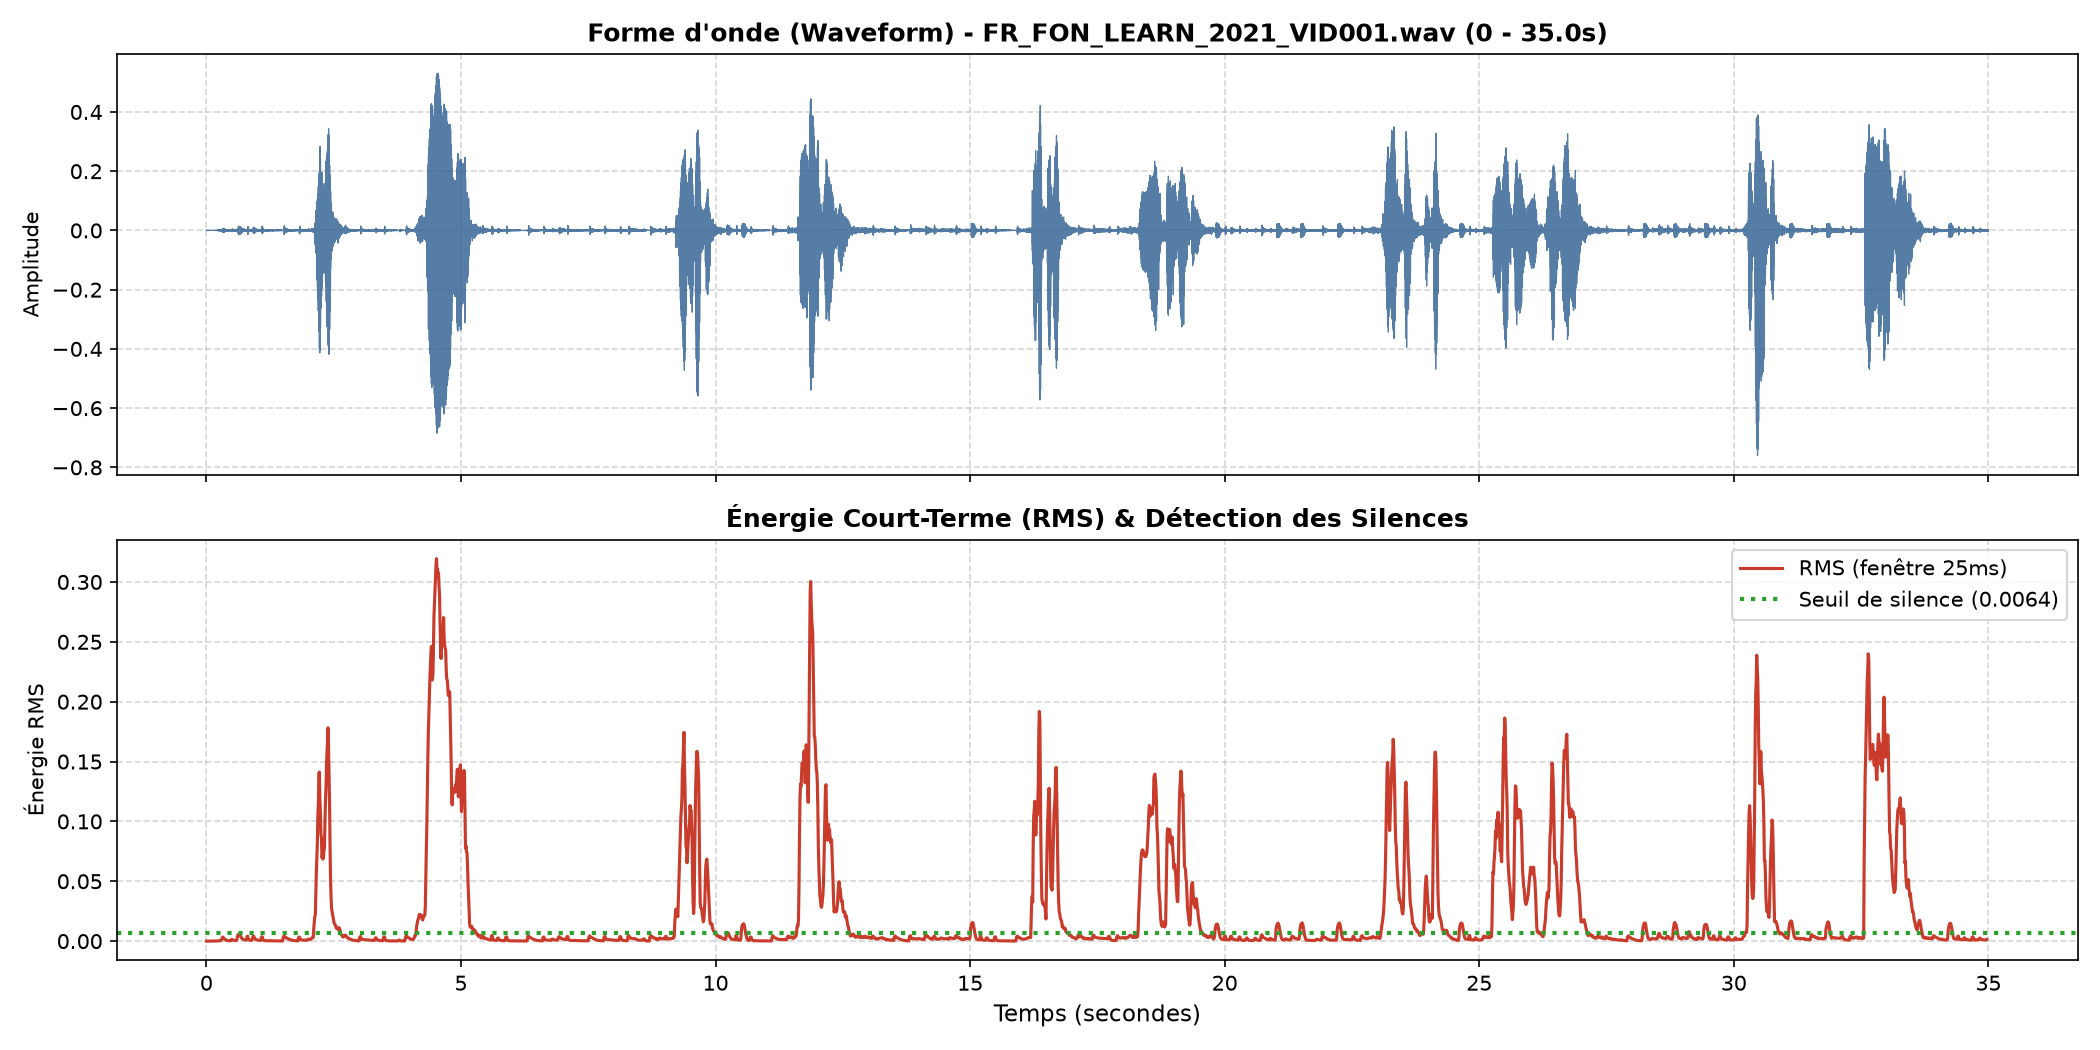
\includegraphics[width=0.88\textwidth,height=0.48\textheight,keepaspectratio]{../figures/waveform_energy_VID001.png}
\end{center}
\vspace{-0.2cm}
\begin{itemize}
    \item \textbf{Alternance temporelle nette :} $S_1$ (Français : \textit{"Bonjour !"}) $\rightarrow$ Silence $\rightarrow$ $T_1$ (Fongbe : \textit{"Dóo núwe"}).
    \item \textbf{Résultat de découpage :} \textbf{127 segments vocaux unitaires} extraits avec succès, sans fausses alertes.
\end{itemize}
\end{frame}

% ------------------------------------------------------------------------------
% SLIDE 7 : ANALYSE D'INCIDENTS TECHNIQUES
% ------------------------------------------------------------------------------
\begin{frame}{6. Incidents Techniques Résolus (Ingénierie \& Acoustique)}
\small
\begin{table}[h]
\centering
\begin{tabular}{p{3.5cm}p{4.2cm}p{4.5cm}}
\toprule
\textbf{Incident rencontré} & \textbf{Cause racine} & \textbf{Solution déployée} \\
\midrule
Échec de build \texttt{llvmlite} sur macOS Intel & Incompatibilité Python 3.14 (pré-release sans wheels x86\_64). & Environnement virtuel verrouillé en \textbf{Python 3.11} via \texttt{uv}. \\
\addlinespace
Blocage binaire FFmpeg & Homebrew arrêté en \textit{Tier 3} sur l'OS hôte. & Intégration du package autonome \textbf{\texttt{imageio-ffmpeg}}. \\
\addlinespace
Sous-segmentation ($44\,\text{s}$) et faux silences & Seuil percentile aveugle capturant le souffle du micro. & Algorithme adaptatif \textbf{Top-dB ($26\,\text{dB}$ sous le pic RMS)}. \\
\bottomrule
\end{tabular}
\end{table}
\end{frame}

% ------------------------------------------------------------------------------
% SLIDE 8 : PERSPECTIVES PHASE 2 & CONCLUSION
% ------------------------------------------------------------------------------
\begin{frame}{7. Intégration du Corpus FFR-v1 \& Feuille de Route Phase 2}
\begin{columns}[T]
    \begin{column}{0.5\textwidth}
        \textbf{Le rôle pivot de FFR-v1 (Dossou et al.) :}
        \begin{itemize}
            \item 117\,000 phrases parallèles Français--Fongbe.
            \item Calibre la loi du \textbf{ratio de durée} ($\mu_r \approx 1{,}1$, $\sigma_r \approx 0{,}3$).
            \item Sert de lexique de référence avec gestion stricte des diacritiques.
        \end{itemize}
        \vspace{0.1cm}
        \textbf{Baseline Mathématique Phase 2 :}
        $$\operatorname{Score}(S_i, T_j) = w_1 T + w_2 D + w_3 P + w_4 A$$
    \end{column}
    \begin{column}{0.5\textwidth}
        \begin{block}{Jalons de Novembre (Phase 2)}
            \begin{enumerate}
                \item Génération des paires candidates $(S_i, T_j)$ par fenêtre glissante.
                \item Évaluation de la baseline analytique explicable.
                \item Entraînement de classificateurs supervisés Scikit-learn (Random Forest, SVM, Régression Logistique).
            \end{enumerate}
        \end{block}
        \vspace{0.2cm}
        \centering
        \textbf{\color{amablue}Phases 0 \& 1 validées -- Prêts pour la modélisation ML !}
    \end{column}
\end{columns}
\end{frame}

\end{document}